\documentclass[a4paper,11pt,parskip,abstract=on]{scrartcl}
\usepackage[utf8]{inputenc}
\usepackage[ngerman]{babel}
\usepackage[T1]{fontenc}
\usepackage{lmodern}
\usepackage{amsmath}
\usepackage{amsfonts}
\usepackage{amssymb}
\usepackage{amsthm}
\usepackage{siunitx}
\usepackage{epsfig}
\usepackage{url}
\usepackage{tikz}
\usepackage[lined,algoruled,linesnumbered]{algorithm2e}
%% \usepackage{algpseudocode}
%% \usepackage{algorithm}
\usepackage{graphicx}
\usepackage{placeins}

% an seitenbreite angepasste tabellen
\usepackage{booktabs}
\usepackage{tabularx} % page-width
\usepackage{adjustbox}

% coole inline-todos :)
\usepackage[colorinlistoftodos,prependcaption]{todonotes}

% Zeilenabstand
\usepackage[onehalfspacing]{setspace}

% Überschriftenabstand
\usepackage{titlesec}
\titlespacing\section{0pt}{12pt plus 4pt minus 2pt}{-5pt plus 2pt minus 2pt}
\titlespacing\subsection{0pt}{12pt plus 4pt minus 2pt}{-5pt plus 2pt minus 2pt}
\titlespacing\subsubsection{0pt}{12pt plus 4pt minus 2pt}{-5pt plus 2pt minus
2pt}

% PDF Bookmarks
\usepackage[backref=true,pagebackref=true,colorlinks=false,bookmarks=true,bookmarksopen=false,bookmarksnumbered=false,pdfpagemode=None]{hyperref}

% Seitenränder
\usepackage{geometry}             % Satzspiegel festlegen
\geometry{left=3cm, right=2.5cm, top=3cm, bottom=2cm, foot=1cm}

% Typographie: Besseres Absatz-Handling, größere Toleranzen beim Blocksatz
\tolerance 1414
\hbadness 1414
\emergencystretch 1.5em
\hfuzz 0.3pt
\widowpenalty=10000               % Hurenkinder vermeiden
\displaywidowpenalty=10000        % Hurenkinder vermeiden
\clubpenalty=10000                % Schusterjungen vermeiden
\vfuzz \hfuzz
\raggedbottom

\renewcommand{\arraystretch}{1.5}

\usetikzlibrary{shapes.geometric, positioning, calc, shapes, fit, backgrounds}

\title{Projektausarbeitung \\\vspace{.5cm} \large gt Scaffolder: Eine Scaffolding-Software}

\author{Dorle Osterode, Lukas Götz \& Stefan Dang}
\date{}

\begin{document}
\maketitle{}
\thispagestyle{empty}
\begin{abstract}
gt Scaffolder ist eine Scaffolding-Software, welche auf der Infrastruktur der
GenomeTools-Bibliothek aufbaut und sich methodisch an SGA Scaffold anlehnt.
Die Scaffold-Berechnung erfolgt mithilfe eines Scaffold-Graphen, welcher
reduziert und traversiert wird. Für 4 Testdatensätze wurden mit SGA
vergleichbare Ergebnisse erzielt -- bei gleichzeitig geringerem Zeit- und
Speicherplatzbedarf.
Diese Projektausarbeitung erläutert die für die Implementation
von gt Scaffolder benötigten Algorithmen und Datenstrukturen und diskutiert
die erzielten Ergebnisse.
\end{abstract}

\newpage{}
\thispagestyle{empty}
\tableofcontents{}
\newpage{}
\setcounter{page}{1}
\section{Einleitung}

Das Ziel einer DNA-Sequenzierung ist die Bestimmung der Basen-Abfolge
der vorliegenden DNA. Moderne Sequenzierungstechniken, auch
\textit{Next-Generation Sequencing} genannt, können auch Read-Paare
produzieren. Dabei werden jeweils beide Enden eines DNA-Fragments
sequenziert. Abhängig vom verwendeten Sequenzierungsprotokoll
überbrücken gepaarte Reads Lücken (Inserts) variabler Größe.

Zur Rekonstruktion der Zielsequenz aus den Reads unabhängig von einer
Referenzsequenz kann eine \textit{de novo} Assemblierung durchgeführt
werden. Typischerweise wird hierbei in zwei Schritten vorgegangen:
Zunächst werden die einzelnen Reads zu durchgängigen Sequenzen
(Contigs) assembliert. Dabei kann das Zielgenom oftmals nicht
vollständig rekonstruiert werden. Aufgrund teilweise unzureichender
Abdeckung durch die Sequenzierung sowie repetitiver Teilsequenzen
entstehen Lücken (Gaps), welche zu unabhängigen Contigs führen. Die
relative Anordnung und Orientierung der Contigs zueinander kann nicht
bestimmt werden.

Durch \textit{Paired-End}- oder \textit{Mate-Pair}-Sequenzierung
gewonnene Read-Paare können auf unterschiedlichen Contigs liegen und
so eine Beziehung zwischen diesen herstellen. Im zweiten Schritt einer
\textit{de novo} Assemblierung können diese Distanzinformationen dazu
verwendet werden, um die Contigs in Scaffolds anzuordnen. Dies erhöht
den Zusammenhang der assemblierten Sequenz. Scaffolds bestehen
dabei aus einer Reihe von geordneten Contigs, deren Distanz und
relative Orientierung festgelegt werden.

Das Scaffolding Problem kann als graphentheoretisches Problem formuliert
werden. Dabei repräsentieren die Knoten des Graphen die einzelnen Contigs.
Zwischen zwei Knoten existiert eine Kante, falls ein Read-Paar die beiden
repräsentierten Contigs verbindet. Kanten enthalten hierbei Informationen über
die Distanz der verbundenen Contigs und die Orientierung der Read-Paare
zueinander. Die Ermittlung eines Scaffolds bzw.\ eines optimalen Pfades (Pfad
mit maximalem Kantengewicht) jeder Zusammenhangskomponente des Scaffold-
Graphen, ist NP-vollständig~\cite{Huson:2002kf}. Daher wird häufig eine
Heuristik verwendet, um einen guten Pfad zu bestimmen.

Diese Ausarbeitung beschäftigt sich mit der Implementation eines
Scaffolding-Programms im Rahmen des Genominformatik-Projektes. Die
Implementation und komplette Dokumentation ist unter
\url{https://github.com/dorleosterode/gt-scaffold} zu finden. Der Fokus dieser
Ausarbeitung liegt auf der zugrunde liegenden Methodik. Für
Implementationsdetails steht der Source Code zur Verfügung.

\section{Ziel des Projektes und Vorgehen}
\subsection{Ziel des Projektes}
Die Implementierung und Evaluierung einer Scaffolding-Software stellte
das allgemeine Projektziel dar. Dabei sollten die in der
GenomeTools-Bibliothek~\cite{Gremme:2013} vorhandenen Konzepte und
Infrastruktur verwendet und eine Kompatibilität mit den Ausgaben des
Assemblers Readjoiner~\cite{Gonnella:2012gn} gewährleistet werden. Der
Scaffolder aus dem SGA-Softwarepaket~\cite{Simpson:2012ef} sollte als
Vorlage dienen, da diese Software im Rahmen einer Untersuchung
verschiedener Scaffolding-Programme gute Ergebnisse
lieferte~\cite{Hunt:2014dh}. Andererseits enthält SGA Scaffold
zahlreiche Abhängigkeiten zu nicht-Standardsoftware, die durch die
Reimplementierung minimiert werden sollten. Dazu gehört zum Beispiel,
dass zur Ermittelung der Distanzinformationen eine Zuordnung der Reads
zu den Contigs auf Basis des String-Graphen erfolgen kann anstelle eines
Read-Mappings durch z.\,B. BWA~\cite{Li:2009}. Des Weiteren existiert keine
hinreichende Dokumentation der Methodik von SGA Scaffold, so dass
dessen Aufklärung einen zentralen Teil des Projektes umfasste.

\subsection{Vorgehen}
Die erste Aufgabe bestand darin, die Datenformate und Algorithmen
von SGA Scaffold aufzuklären. Die benötigten Informationen
wurden direkt aus dem Quelltext von SGA extrahiert, der über die
Plattform GitHub frei zugänglich ist~\cite{source}.

Die Datenformate und Algorithmen wurden leicht modifiziert und in
der Programmiersprache C neu implementiert, um sowohl Laufzeit
als auch Speicherplatz einzusparen. Mehrere Unklarheiten in der
Methodik wurden zunächst übernommen, um die gleichen Resultate wie
SGA Scaffold erzeugen zu können. Des Weiteren verwendeten wir die
Eingabeformate von SGA Scaffold, damit die Ergebnisse von gt Scaffolder
und SGA Scaffold verglichen werden konnten.

Als nächstes simulierten wir eine \textit{Paired-End}-Sequenzierung mit
einem Illumina Sequenzierer für verschiedene Referenzsequenzen
(\textit{S. cerevisiae}, \textit{H. sapiens}, \textit{C. elegans}
 \textit{D. melanogaster}) durch die Software ART~\cite{Huang:2012kq}.
Danach wurde eine Genomassemblierung für die \textit{Paired-End}
Bibliotheken mit der SGA-Pipeline und der Scaffolding-Schritt
mit gt Scaffolder und SGA Scaffold durchgeführt. Schließlich erfolgte
eine Evaluation der Ergebnisse.

\section{Methoden}
\label{sec: Methoden}

\subsection{Algorithmen}
\subsubsection{Übersicht der Schritte}

\begin{figure}
  \centering
    \begin{tikzpicture}[every node/.style={font=\footnotesize}]
    \node[] (input1) {Contigs};
    \node[left of=input1, xshift=-1cm] (eingabe) {\textbf{Eingabe:}};
    \node[below of=eingabe, yshift=-5cm] (ausgabe) {\textbf{Ausgabe:}};
    \node[right of=input1, align=center, xshift=2cm] (input2) {Distanz-\\informationen};
    \node[right of=input2, xshift=2cm] (input3) {A-Statistik};

    \node[below of=input1, yshift=-.5cm, anchor=west] (titel) {gt Scaffolder};
    \node[rectangle, draw, anchor=west, below of=titel, xshift=1cm, rounded corners, fill=black!10, yshift=.25cm] (konstruktion) {Konstruktion des Graphen};
    \node[rectangle, draw, anchor=west, below of=konstruktion, xshift=.95cm, rounded corners, fill=black!10, yshift=.25cm] (selektion) {Selektion relevanter Knoten und Kanten};
    \node[rectangle, draw, anchor=west, below of=selektion, xshift=.80cm, rounded corners, fill=black!10, yshift=.25cm] (ermittlung) {Ermittlung aller Zusammenhangskomponenten (ZK)};
    \node[rectangle, draw, anchor=west, below of=ermittlung, xshift=-.65cm, rounded corners, fill=black!10, yshift=.25cm] (pfade) {Bestimmung des besten Pfades für jede ZK};

    \begin{pgfonlayer}{background}
    \node[draw, fit={(titel) (konstruktion) (selektion) (ermittlung) (pfade)}, rounded corners, fill=black!20] (back) {};
    \end{pgfonlayer}

    \node[below of=back, yshift=-2cm, xshift=-1.5cm] (output1) {Scaffolds};
    \node[right of=output1, align=center, xshift=2cm, yshift=-.25cm] (output2) {(rekonstruierte\\Sequenzen)};
    \node[above of=output1] (dummy) {};

    \path[->, thick]
    (input1) edge (back)
    (input2) edge (back)
    (input3) edge (back)
    (back) edge (output1)
    (back) edge (output2);
  \end{tikzpicture}
    \caption{\label{abb: gtscaffolder}Schematische Darstellung des Programmablaufs von gt Scaffolder.}
\end{figure}

In Abbildung~\ref{abb: gtscaffolder} ist der Programmablauf von gt
Scaffolder schematisch dargestellt. Als Eingabe dienen Dateien, die
die Repetitivität, die Sequenz und die Distanzinformationen der
einzelnen Contigs beschreiben. Mit Hilfe dieser Eingaben erfolgt
zunächst die Konstruktion des Scaffold-Graphen. Im Anschluss werden
die relevanten Knoten und Kanten selektiert und alle
Zusammenhangskomponenten des Scaffold-Graphen ermittelt.  Danach wird
für jede Zusammenhangskomponente ein Pfad berechnet, der als Scaffold
ausgegeben wird.

Die einzelnen Schritte werden in den folgenden Abschnitten näher erläutert.

\subsubsection{Eingabe}
Als Eingabe werden die Contigs im FASTA-Format, die
Distanzinformationen aus der \textit{Paired-End}-
bzw. \textit{Mate-Pair}-Sequenzierung und die A-Statistik der einzelnen
Contigs benötigt.

In gt Scaffolder können die Distanzinformationen explizit durch eine
Datei im ABySS-Distanz-Format (*.de) angegeben werden. Eine solche
Datei wird durch das Programm DistEst von ABySS~\cite{abyss} nach der Assemblierung
und dem Read-Mapping in der SGA-Pipeline erstellt und dient als
Eingabe der Distanzinformationen für SGA Scaffold. In der Evaluierung
wurde diese Option für Vergleiche zwischen gt Scaffolder und SGA Scaffold
verwendet. Des Weiteren besteht die Möglichkeit, die Distanzinformationen aus
einer Datei im BAM-Format (*.bam) mit Hilfe eines Moduls zu
extrahieren. Dafür diente die Methode des Programms DistEst von ABySS
als Vorlage. Aus Zeitgründen ist es nicht gelungen ein Modul zu
entwickeln zur Erzeugung der BAM-Datei auf Basis des String-Graphen.
Stattdessen muss ebenfalls ein Read-Mapping separat nach der Assemblierung
durchgeführt werden.

Die A-Statistik ist ein statistisches Maß und beschreibt die Repetitivität
einer Sequenz~\cite{Myers:2005iq}. Die A-Statistik kann in Form einer
separaten Datei oder als Annotation in den Contigs angeführt werden.

\subsubsection{Erstellen der Distanzinformationen}
Die Methode, die das Programm DistEst verwendet, durchläuft folgende
Schritte. Zunächst werden alle Reads aus der BAM-Datei geladen und
die Read-Paare ermittelt. Anschließend werden die Fragmentlängen
aller Read-Paare berechnet, die gegenüber dem gleichen Contig angeordnet sind,
und auf deren Basis eine Häufigkeitsverteilung erstellt.
Danach wird aus der Verteilung eine Wahrscheinlichkeitsfunktion für die
Fragmentlängen abgeleitet. Im nächsten Schritt versucht man, den paarweisen
Abstand der Contigs durch eine Maximum-Likelihood-Methode abzuschätzen.
Dabei werden für ein Contig-Paar die zugehörigen Read-Paare ermittelt und
deren Fragmentlänge berechnet unter der Annahme, dass die beiden Contigs
ohne Lücke direkt aneinander angrenzen. Als nächstes werden mehrere
Iterationen durchlaufen, bei denen jeweils die Fragmentlängen um einen Faktor (min\_dist
bis max\_dist) korrigiert werden. Des Weiteren erfolgt eine Aufsummierung
der logarithmischen Wahrscheinlichkeiten (log odds) der korrigierten
Fragmentlängen multipliziert mit dessen Häufigkeiten in jedem Durchlauf.
Schließlich wählt man als Abstand zwischen den Contigs den Faktor, bei
dem die Summe der Wahrscheinlichkeiten ein Maximum erreicht.
\todo{Strangorientierung fehlt}

\subsubsection{Konstruktion des Graphen}
Aus den Contigs und den Distanzinformationen wird der Scaffold-Graph
konstruiert. Dabei wird für jeden Contig, der eine Mindestlänge von
200 bp überschreitet, eine A-Statistik größer 19 und eine berechnete
Anzahl an Kopien von mindestens \num{0.3} hat, ein Knoten in den Graph
eingefügt. Die Distanzinformationen werden genutzt um die Knoten durch
Kanten miteinander zu verbinden. Dabei werden zwischen jedem Paar von
Knoten, zwischen dessen repräsentierten Contigs eine
Distanzinformation anhand von Read-Paaren vorhanden ist, zwei Kanten
eingefügt. Die Kanten geben jeweils Orientierung und Distanz an.

\subsubsection{Selektion relevanter Knoten und Kanten}
In dem konstruierten Graph werden relevante Knoten und Kanten
selektiert. Dazu werden nicht relevante Knoten und Kanten markiert und
im späteren Vorgehen nur unmarkierte Knoten und Kanten betrachtet. Es
werden folgende Kriterien überprüft:
\begin{itemize}
\item Polymorphe Knoten: Zwei Knoten gelten als polymorph, wenn diese
  sich bezüglich eines gemeinsamen Vorgängerknotens anhand ihrer
  Distanz nicht eindeutig anordnen lassen. Zusätzlich muss die
  Kopiezahl beider Knoten gering genug sein. Der Knoten mit der
  geringeren Kopiezahl und dessen eingehenden und ausgehenden Kanten
  werden als polymorph markiert und nicht weiter betrachtet.
\item Inkonsistente Kanten: Zwei Kanten $e_1$ und $e_2$ gelten als
  inkonsistent, wenn sich die Endknoten $e_1.end$ und $e_2.end$ bei
  einer Anordnung anhand ihrer Distanz bezüglich des gemeinsamen
  Startknotens $e_1.start = e_2.start$ mit mindestens 400 bp
  überlappen. Gehen von einem Knoten zwei inkonsistente Kanten aus, so
  werden alle ausgehenden Kanten des Knotens sowie ihre Rückkanten als
  inkonsistent markiert. Zusätzlich werden alle Kanten der über
  inkonsistente Kanten erreichbaren Knoten, die die gleiche Richtung
  (\textit{sense} oder \textit{antisense}) wie die markierte Rückkante
  haben, als inkonsistent markiert. Alle markierten Kanten werden
  nicht weiter betrachtet.
\end{itemize}
Der Pseudocode zur Markierung polymorpher Knoten und inkonsistenter
Kanten ist in Algorithmus \ref{alg: Selektion} dargestellt.

Zusätzlich werden gerichtete Zyklen aufgelöst. Dazu werden alle
Zusammenhangskomponenten des Graphen berechnet. Für jede dieser
Zusammenhangskomponenten wird mit einer rekursiven Tiefensuche nach
Rückkanten gesucht. Dabei wird diese Tiefensuche von jedem terminalen
Knoten, ein Knoten der nur ausgehende \textit{sense} oder
\textit{antisense} Kanten hat, aus gestartet. Wird eine Rückkante
gefunden, so werden die Kante und die durch die Kante verbundenen
Knoten als zyklisch markiert und nicht weiter betrachtet. Da sich
durch die Entfernung von Kanten und Knoten die Struktur des Graphen
verändert und immer nur ein Zyklus für jeden terminalen Knoten
aufgelöst wird, muss diese Prozedur so lange wiederholt werden bis
keine Zyklen mehr gefunden werden.

Der Pseudocode für die Detektion und das Auflösen von Zyklen ist in
Algorithmus \ref{alg: Zyklen} abgebildet.

\subsubsection{Ermittlung des besten Pfades (Scaffolding)}

Nach der Selektion relevanter Knoten und Kanten wird das eigentliche
Scaffolding durchgeführt. Dazu werden alle Zusammenhangskomponenten
des Graphen bestimmt, um für jede Zusammenhangskomponente die beste
Anordnung der repräsentierten Contigs zu berechnen. Für jede
Zusammenhangskomponente werden die kürzesten Pfade bezüglich der
Kantengewichte zwischen allen terminalen Knoten mit einer Breitensuche
berechnet. Der kürzeste Pfad mit der meisten Sequenzabdeckung wird als
Scaffold für die Zusammenhangskomponente gewählt. Die Sequenzabdeckung
eines Pfades berechnet sich dabei durch die Aufsummierung der
Sequenzlängen der enthaltenen Contigs.

Contigs, deren repräsentierende Knoten keine oder nur markierte Kanten
haben, werden ebenfalls als Scaffolds gewählt.

Der Pseudocode für die Berechnung des Scaffolds ist in Algorithmus
\ref{alg: Scaffold} dargestellt.

\subsubsection{Ausgabe}
Die ermittelten Scaffolds werden in dem gleichen Format ausgegeben,
wie bei SGA. In diesem Format (*.scaf) steht in jeder Zeile
ein Scaffold. Die einzelnen Contigs mit ihren Informationen sind dabei
durch Tabs getrennt. Ein Beispieleintrag ist in Abbildung \ref{abb:
  scaf} dargestellt. Der erste Eintrag in einer Zeile ist die ID des
Startcontigs. Für die darauffolgenden Contigs werden folgende
Informationen durch Kommata getrennt angegeben: ID des Contigs, Distanz
zu dem vorherigen Contig, Standardabweichung der Distanz, Orientierung
zu dem vorherigen Contig (0: gleicher Strang, 1: entgegengesetzter
Strang) und Information über die Lage des Reads aus dem Read-Paar (0:
gleicher Strang, 1: entgegengesetzter Strang).

\begin{figure}
\begin{verbatim}
contig-100070  contig-34044,-99,2.500000,0,1,  contig-29023,-23,3.700000,0,0,
\end{verbatim}
\caption{\label{abb: scaf}Beispielzeile aus der Ausgabe von gt
  Scaffolder für den \textit{C. elegans} Testdatensatz.}
\end{figure}

Zusätzlich wurde ein Modul geschrieben um die Sequenzen der
berechneten Scaffolds rekonstruieren zu können. Bei SGA ist dies
ebenfalls ein separater Schritt. Um die Sequenzqualität zu verbessern
wird dabei versucht Überlappungen durch Sequenzalignments aufzulösen
und Lücken zwischen den Contigs durch Pfade im String-Graph zu
schließen. Die Rekonstruktion der Sequenzen ist in Abschnitt \ref{sec:
  Rekonstruktion} näher beschrieben und wurde separat evaluiert (siehe
Abschnitt \ref{sec: Seq-Rek}).

\subsubsection{Rekonstruktion der Sequenz}
\label{sec: Rekonstruktion}
Zur Rekonstruktion der Sequenzen der berechneten Scaffolds werden drei
Schritte für alle aufeinander folgende Contigs durchlaufen. Zuerst
wird versucht die Lücke zwischen den Contigs anhand eines Pfades
in dem String-Graph zu schließen. Für diesen Schritt wird der
String-Graph aller Contigs verwendet. Konnte kein eindeutiger Pfad nach
bestimmten Kriterien gefunden werden, so wird überprüft, ob die
Contigs sich überlappen. Ist die Distanz zwischen den Contigs negativ,
werden die sich überlappenden Enden aligniert. Wenn kein Alignment
gefunden wurde, wird die Lücke mit Wiederholungen des Buchstaben 'N'
aufgefüllt.

Die gesamte Sequenz eines Scaffolds wird anhand dieser drei Schritte
folgendermaßen rekonstruiert. Die komplette Sequenz des ersten Contigs
wird übernommen. Danach wird für den jeweils nächsten Contig versucht
einen eindeutigen Pfad der richtigen Länge zwischen dem vorherigen und
diesem Contig im String-Graph zu finden. War dies nicht erfolgreich
wird bei negativer Distanz versucht zwischen den Contigs ein Alignment
zu finden. Ansonsten wird die Lücke zwischen den Contigs mit einer Reihe
von 'N'-Symbolen aufgefüllt. Bei diesem Vorgang wird die relative
Orientierung der Contigs zueinander und zum ersten Contig
beachtet. Dementsprechend wird jeweils die normale, die reverse oder
revers-komplementäre Sequenz verwendet.

\paragraph{Traversierung des String-Graphen}~\\
Nach der Assemblierung wird in SGA ein String-Graph im ASQG-Format
(*.asqg) ausgegeben. Für eine Beschreibung des Formats
siehe~\cite{asqg}. Dieser String-Graph wird mit einem Python-Skript in
das SPM-Format (*.spm) umgeschrieben. Das SPM-Format wird von
Readjoiner verwendet um String-Graphen zu repräsentieren.

Wie in Abbildung \ref{abb: spm} dargestellt, ist das SPM-Format ein
zeilenbasiertes Format. In jeder Zeile ist eine Suffix-Präfix-Überlappung
eingetragen. Die erste Zahl repräsentiert den einen Contig oder Read,
das folgende Zeichen gibt den Strang an ('+' steht für den
\textit{sense}-Strang und '-' für den \textit{antisense}-Strang), die
zweite Zahl repräsentiert den zweiten Contig oder Read, das folgende
Zeichen gibt den Strang an und die letzte Zahl entspricht der Länge
der Überlappung. Die Zahlen für die Contigs oder Reads entsprechen
dabei der Sequenznummer des Contigs oder Reads in einer GtEncseq,
einer komprimierten Sequenzrepräsentation in den GenomeTools.

\begin{figure}
  \centering
\begin{verbatim}
24129 + 0 + 148
1 + 85225 - 123
39261 - 1 + 137
2 + 27698 + 149
\end{verbatim}
\caption{\label{abb: spm}Beispielzeilen aus der .spm-Datei des
  String-Graphen für den \textit{C. elegans} Testdatensatz.}
\end{figure}

Aus dieser Repräsentation wird der String-Graph nach der Assemblierung
wieder aufgebaut. Dazu wird die Datei im SPM-Format mit Infrastruktur
eingelesen, die in den Readjoiner zugrunde liegenden Bibliotheken
vorhanden ist.

Der String-Graph wird anschließend für jedes Paar
aufeinanderfolgender Contigs $c_1$, $c_2$ in jedem Scaffold mit einer
Breitensuche traversiert. Es wird versucht einen eindeutigen Pfad von
Contig $c_1$ zu Contig $c_2$ in dem String-Graph zu finden. Dabei wird
überprüft, ob die Distanz zwischen den Contigs die im Scaffolding
ermittelte Distanz nicht überschreitet. Um eine Traversierung des
gesamten String-Graphen zu verhindern, wird die Suche nach \num{10000}
besuchten Knoten abgebrochen. Ein gefundener Pfad wird dabei
verworfen, da die Eindeutigkeit nicht garantiert werden kann. Wird
mehr als ein Pfad zwischen den Contigs gefunden, wird die Suche
ebenfalls ohne Ergebnis abgebrochen.

Wurde ein eindeutiger Pfad gefunden, so wird der Pfad von $c_1$ zu
$c_2$ gespeichert und anschließend die Sequenz des Pfades anhand der
Repräsentation der Sequenzen der Contigs als GtEncseq rekonstruiert.
Diese rekonstruierte Sequenz wird schließlich zurückgegeben.

\paragraph{Berechnung von Alignments}~\\
Ist die Distanz zwischen zwei im Scaffold benachbarten Contigs $c_1$
und $c_2$ negativ, so überlappen sich die Contigs. Um diese
Überlappung in der Sequenz aufzulösen, wird ein Alignment zwischen den
Contigs $c_1$ und $c_2$ berechnet. Dabei wird das beste Alignment
genutzt, um die Sequenz zu rekonstruieren.

Es wird eine in den GenomeTools schon vorhandene Implementation des
Smith-Waterman-Algorithmus für lokale Alignments~\cite{smith}
verwendet. Der Sequenzbereich der Contigs, in dem Alignments gesucht
werden, wird dabei durch die im Scaffolding ermittelte Distanz und das
dreifache der Standardabweichung festgelegt. Der Sequenzbereich wird
zusätzlich durch die Längen der beiden Contigs eingeschränkt. Maximal
werden allerdings je 500 Basen zur Berechnung des Alignments
verwendet, um zu hohen Rechenaufwand zu vermeiden. Diese Maximallänge
wurde von SGA übernommen.

Nur Suffix-Präfix-Überlappungen von Contig $c_1$ mit Contig $c_2$
werden betrachtet, wenn Contig $c_1$ im Scaffold direkt vor Contig
$c_2$ kommt. Die maximale erlaubte Fehlerrate (für Sequenzen $u$ und
$v$ und die maximale Edit-Distanz $max\_edist$ ergibt sie sich aus:
$max\_error = max\_edist \cdot \text{MAX}(u,v)$) ist $max\_error =
0.05$ nach dem standardmäßig bei SGA verwendeten Wert. Ebenso wurde
die Mindestlänge eines Alignments auf 20 Basen festgelegt.

Von allen gefundenen, den Kriterien entsprechenden Alignments, wird das
Alignment mit der kleinsten Edit-Distanz gewählt. Ist $l$ die Länge
des besten Alignments und $seq_{c_2}$ die Sequenz des Contigs $c_2$,
so wird die Sequenz ab der Position $l$ ($seq_{c_2}[l,|seq_{c_2}|]$)
zurückgegeben. Falls kein hinreichendes Alignment gefunden werden
konnte, muss der nächste Schritt durchgeführt werden.

\paragraph{Die Lücke zwischen zwei Contigs schließen}~\\
Konnte die Lücke zwischen zwei Contigs $c_1$ und $c_2$ nicht durch
eine Graph-Traversierung oder ein Alignment geschlossen werden, so
wird in diesem Schritt die Sequenz mit Wiederholungen des Buchstaben
'N' aufgefüllt. Dabei gibt es eine Fallunterscheidung anhand der
Distanz.

Ist die ermittelte Distanz zwischen $c_1$ und $c_2$ positiv, so wird
die Sequenz von $c_2$ nicht verändert. Vor die Sequenz werden der
Distanz entsprechend viele 'N'-Symbole geschrieben, jedoch mindestens
25.

Ist die ermittelte Distanz zwischen $c_1$ und $c_2$ negativ, so wird
der Präfix von $c_2$ der Länge 25 durch die gleiche Anzahl an
'N'-Symbolen ersetzt.

\subsection{Datenstrukturen}
\label{sec: Datenstrukturen}

Der GtScaffolderGraph stellt die zentrale Datenstruktur von gt Scaffolder dar
und besteht aus Knoten und Kanten, die über Zeiger miteinander verknüpft sind.
Die Knoten repräsentieren die Contigs und enthalten als Eigenschaften dessen
Header Sequenz, Sequenzlänge, A-Statistik Wert und Kopiezahl. Außerdem
verfügen sie über einen Zustand, der die Klassifikation des Knotens beschreibt
(z.\,B. polymorphe oder repetitive Knoten), und besitzen Zeiger auf ihre ausgehenden
Kanten.

Die Kanten stellen die Distanzinformationen zwischen den Contigs dar und
enthalten als Eigenschaften den paarweisen Abstand, deren Standardabweichung,
die Anzahl der Read-Paare, die zur Abstandsberechnung verwendet wurden und die
Strangorientierung der beteiligten Contigs und Reads. Des Weiteren besitzen sie einen
Zustand, der die Klassifikation der Kante beschreibt (z.\,B. inkonsistente oder
polymorphe Kanten) und Zeiger auf die beteiligten Contigs.

Die Module Parser und Algorithms benutzen den Graph. Der Parser liest
die Informationen für die Contigs aus der Datei im FASTA-Format und
die Distanzinformationen aus der entsprechenden Datei ein und
allokiert und befüllt den Graph dementsprechend. Das Modul für die
Algorithmen benutzt die so konstruierte Graph-Struktur um die in
Abschnitt \ref{sec: Methoden} dargestellten Berechnungen
durchzuführen. Dazu gehören die Selektion der relevanten Kanten und
Knoten und das Scaffolding an sich. Zusätzlich wird in dem Modul die
Klassifikation anhand der A-Statistik und die Kopiezahlen für die
einzelnen Contigs durchgeführt, wenn eine separate Datei mit diesen
Informationen übergeben wird. Beide Module haben eine transitive
Abhängigkeit von den Knoten und Kanten.

Die Beziehungen zwischen diesen Modulen ist in Abbildung \ref{abb:
  UML} anhand eines UML-Diagramms dargestellt.

Wie in Abbildung \ref{abb: UML} erkenntlich ist, hat das Modul
Bamparser keinerlei Abhängigkeiten zu den anderen Modulen. Mit diesem
Modul werden die Distanzinformationen generiert, wenn eine Datei im
BAM-Format übergeben wird. Da es keine Abhängigkeiten zu anderen
Modulen gibt, könnte der Bamparser auch als selbständiges Tool in die
GenomeTools aufgenommen werden.

Das Modul zur Rekonstruktion der Sequenzen ist abhängig von dem
Algorithms Modul, da es eine bestimmte Repräsentation der Scaffolds
erwartet. Ansonsten hält es Abhängigkeiten zu den Knoten und Kanten
aber nicht zum Graph.

\begin{figure}
  \centering
  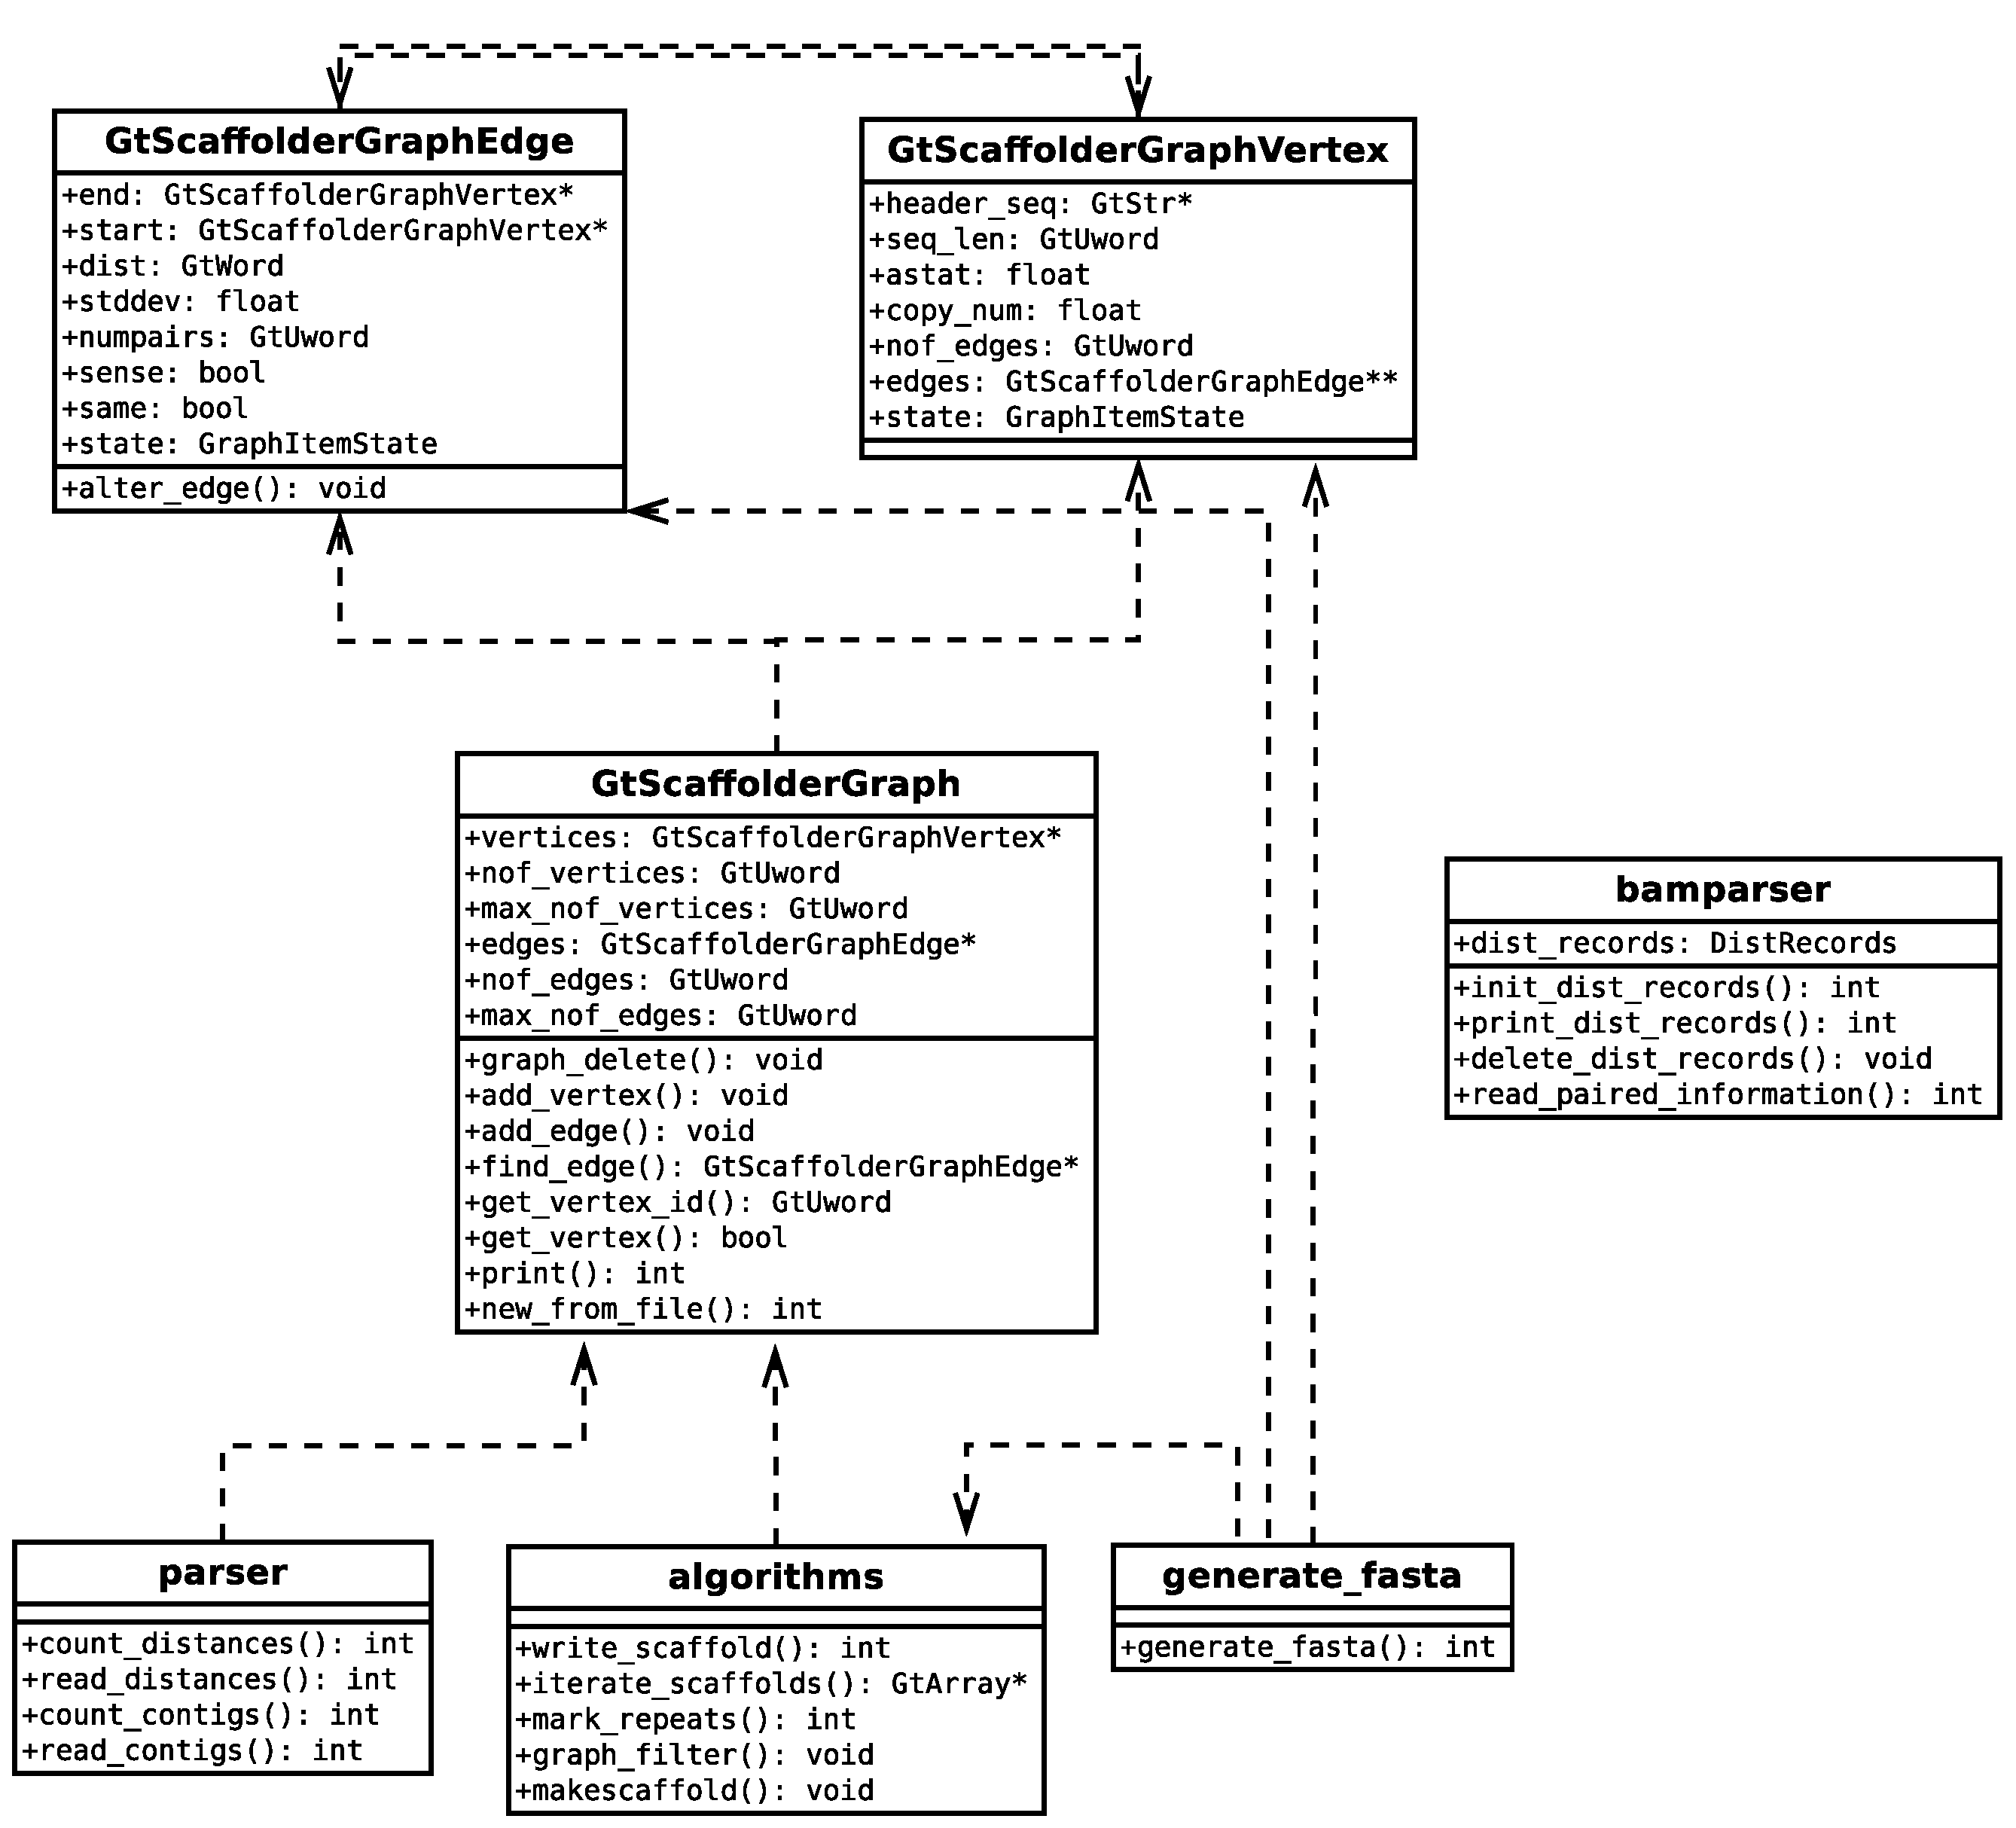
\includegraphics[width=1\linewidth]{uml2.eps}
  \caption{Klassendiagramm für gt Scaffolder.}
\label{abb: UML}
\end{figure}

\subsection{gt Scaffolder als Tool in den GenomeTools}
Die Software gt Scaffolder wurde als eigenständiges Tool in die GenomeTools
eingebunden. In Abbildung \ref{abb: help} ist die Ausgabe der Hilfe des Tools
gt Scaffolder dargestellt, in der alle einstellbaren Parameter mit ihren
standardmäßigen Belegungen aufgelistet sind.

\begin{figure}
\begin{verbatim}
$ gt scaffolder -help
Usage: gt scaffolder [option ...] [file]
Constructs scaffolds of the contigs.

-min_contig_len    minimal contig length for used contigs
                   default: 200
-rep_cp_cutoff     minimal copy number for not repetitiv contigs
                   default: 0.30
-rep_astat_cutoff  minimal A-statistics for not repetitiv contigs
                   default: 20.00
-p_cutoff          probability cutoff for polymorphic vertices
                   default: 0.01
-cp_cutoff         copy num cutoff for polymorphic vertices
                   default: 1.50
-overlap_cutoff    overlap cutoff for inconsistent edges
                   default: 400
-contigs           contigs in FASTA format
                   default: undefined
-dist              distanceinformation in ABySS .de format
                   default: undefined
-astat             A-statistics file in SGAs .astat format
                   default: undefined
-spm               basename of spm-representation of used string-graph
                   default: undefined
-bam_min_qual      minimal quality in bam file
                   default: 10
-bam_min_nof_pairs minimal number of pairs
                   default: 10
-bam_min_dist      minimal distance of contigs
                   default: -99
-bam_max_dist      maximal distance of contigs
                   default: infinite
-bam_min_align     minimal alignment length
                   default: 100
-bam               bam file containing alignments of paired reads to the contigs
                   default: undefined
-help              display help and exit
-version           display version information and exit

Report bugs to <gt-users@genometools.org>.
\end{verbatim}
\caption{\label{abb: help}Hilfeausgabe des Tools gt Scaffolder.}
\end{figure}

Beim Aufruf von gt Scaffolder stellen die Optionen -contig und
entweder -dist oder -bam Pflichtangaben dar. Wenn die Übergabe einer
Distanzdatei im ABySS-Distanz-Format (*.de) mit der Option -dist
erfolgt, dann wird diese Datei eingelesen und die enthaltenen
Distanzinformationen verwendet.  Gibt man dagegen mit der Option -bam
eine BAM-Datei mit Alignments der Reads zu den Contigs an, so werden
aus der BAM-Datei die Distanzinformationen berechnet und im
ABySS-Distanz-Format (*.de) gespeichert. Diese neu erzeugte Datei wird
anschließend eingelesen und die enthaltenen Informationen genutzt.
Die Verwendung einer BAM-Datei und des String-Graph Assemblers
Readjoiner ermöglicht die Abhängigkeit zu einem Mapping-Programm
(z.\,B. BWA) und der Software DistEst von ABySS potentiell zu
durchbrechen. So kann Readjoiner die Positionen der Reads auf den
Contigs direkt ausgeben. Dabei fehlen aber die Information über
Read-Paare und Informationen über enthaltene oder herausgefilterte
Reads. Auf Grund von Zeitmangel existiert jedoch noch kein Modul zur
Konvertierung dieser Daten in eine entsprechende BAM-Datei.

Mit der Option -astat kann zusätzlich eine Datei mit Informationen
über die A-Statistik und die berechneten Kopiezahlen der Contigs
übergeben werden. Diese Option wird für die Kompatibilität mit der
Eingabe von SGA Scaffold benötigt. Wenn diese Option fehlt, besteht die
Annahme, dass diese Informationen innerhalb des Headers der
Contigs vorliegen. Dabei diente das Ausgabeformat für die Contigs von
Readjoiner als Vorlage, das bei Verwendung der Optionen -astat und
-copy$\_$num die A-Statistik und Kopiezahl der Contigs enthält.

Die Standardausgabe stellt eine Datei im SCAF-Format dar. Die
Rekonstruktion der Sequenzen ist in dem Tool noch nicht möglich, da
die Erweiterung der String-Graph-API zur Sequenzkonstruktion mittels
Traversierung des String-Graphen noch nicht in die GenomeTools
übernommen wurde.

\subsection{Strategien in SGA Scaffold mit unklarer Bedeutung}
\label{sec: wunderlich}
SGA benutzt eine relativ konservative Strategie, um vermeintlich
fehlerhafte Knoten und Kanten aus dem Scaffold-Graphen zu
entfernen. Daher werden sehr strikte Schwellenwerte verwendet und
falsch-negative bevorzugt gegenüber falsch-positiven Knoten und Kanten
gelöscht. Einige Strategien von SGA mit unklarer Bedeutung, wurden
zunächst in gt Scaffolder übernommen, um eine Vergleichbarkeit der
Ergebnisse der beiden Programme zu erhalten. Im Folgenden findet sich
eine Auflistung dieser Strategien teilweise kombiniert mit einer
Beschreibung der möglichen Bedeutung. Des Weiteren erfolgte zum Teil
die Evaluierung der Güte dieser Strategien
(siehe Abschnitt~\ref{sec: Ergebnisse}).

\begin{figure}
  \centering
  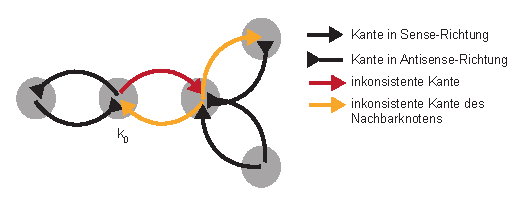
\includegraphics[width=0.6\linewidth]{inkonsistenteKante.eps}
  \caption{Entfernung inkonsistenter Kanten.}
\label{abb: inkonsistenteKante}
\end{figure}

\begin{itemize}
\item Bei der Entfernung inkonsistenter Kanten eines Knotens $k_0$
  werden alle ausgehenden Kanten der Nachbarknoten, die in der gleichen
  Richtung (\textit{sense} oder \textit{antisense}) verlaufen wie die
  Kante vom Nachbarknoten zu $k_0$, ebenfalls als inkonsistent makiert
  und gelöscht (siehe Abbildung~\ref{abb: inkonsistenteKante}).\\
  Mögliche Erklärung: Potentiell enthalten auch diese Kanten
  Inkonsistenzen und sollten deshalb nicht weiter betrachtet werden.
\item Bei der Konstruktion des Graphen werden zwischen zwei Knoten
  jeweils nur zwei Kanten eingefügt, eine Hin- und eine Rückkante.
  Wenn für ein Contig-Paar mehr als eine Distanzinformation existiert,
  also für zwei Knoten mehr als ein mögliches Paar an Kanten vorhanden ist,
  wird das Paar an Kanten mit der größten Standardabweichung gewählt.
  Die Güte dieser Strategie wurde exemplarisch evaluiert
  (vgl. Abschnitt~\ref{sec: wunderlich_assert}).\\
  Mögliche Erklärung: keine.
\item Bei der Klassifikation der Knoten als repetitiv oder eindeutig
  wird neben der A-Statistik auch die berechnete Anzahl an
  Kopien des zugehörigen Contigs betrachtet. Ein Knoten wird
  dabei als repetitiv markiert und später entfernt, wenn die
  A-Statistik oder aber die berechnete Anzahl an Kopien des zugehörigen
  Contigs unterhalb eines Schwellenwertes liegt. \\
  Mögliche Erklärung: Die Contigs mit einer zu geringen
  Kopiezahl sind potentiell fehlerhaft und sollten daher unberücksichtigt
  bleiben. Die Markierung als repetitiv in diesen Fällen ist jedoch
  semantisch inkorrekt und dient nur der späteren Entfernung des
  zugehörigen Knotens.
\end{itemize}

\section{Ergebnisse}
\label{sec: Ergebnisse}
\subsection{Gegenüberstellung der Pipelines}

\begin{figure}
  \centering
  \begin{minipage}{.45\textwidth}
      \begin{tikzpicture}[node distance=.8cm]
        \tikzstyle{prog}=[draw, rectangle, rounded corners];
        \node[prog] (prep) {preprocess};
        \node[prog, below of=prep] (index) {index};
        \node[prog, below of=index] (correct) {correct};
        \node[prog, below of=correct] (index2) {index};
        \node[prog, below of=index2] (filter) {filter};
        \node[prog, below of=filter] (overlap) {overlap};
        \node[prog, below of=overlap] (assemble) {assemble};
        \node[prog, right of=prep, xshift=2.1cm, fill=red!40] (bindex) {index};
        \node[prog, below of=bindex, fill=red!40] (aln) {align};
        \node[prog, below of=aln, fill=red!40] (sampe) {sampe};
        \node[prog, below of=sampe, rectangle split, rectangle split parts=3, yshift=-.45cm, rectangle split part fill={blue!40, green!40, blue!40}] (bam2de) {\nodepart{one}fixmate\nodepart{two}samtools\nodepart{three}DistanceEst};
        \node[prog, below of=bam2de, yshift=-.45cm, fill=yellow!40] (pysam) {astat};
        \node[prog, below of=pysam] (scaff) {scaffold};
        \node[prog, below of=scaff] (scaf2fasta) {scaf2fasta};

        \path[->]
        (prep) edge (index)
        (index) edge (correct)
        (correct) edge (index2)
        (index2) edge (filter)
        (filter) edge (overlap)
        (overlap) edge (assemble)
        (assemble.east) edge[in=180, out=0] (bindex.west)
        (bindex) edge (aln)
        (aln) edge (sampe)
        (sampe) edge (bam2de)
        (bam2de) edge (pysam)
        (pysam) edge (scaff)
        (scaff) edge (scaf2fasta);
      \end{tikzpicture}
    \end{minipage}
    \begin{minipage}{2cm}
      \begin{tikzpicture}[node distance=.8cm]
        \tikzstyle{prog}=[draw, rectangle, rounded corners];
        \node[prog] (prefilter) {prefilter};
        \node[prog, below of=prefilter] (overlap) {overlap};
        \node[prog, below of=overlap] (assembly) {assembly};
        \node[prog, right of=prefilter, xshift=1.5cm] (scaffold) {scaffold};

        \path[->]
        (prefilter) edge (overlap)
        (overlap) edge (assembly)
        (assembly.east) edge[in=180, out=0] (scaffold.west);
      \end{tikzpicture}
    \end{minipage}
    \caption{\label{abb: Pipeline}Assemblierungs- und
      Scaffolding-Pipelines von SGA (links) und gt Scaffolder
      (rechts). Externe Abhängigkeiten zu unterschiedlichen Programmen
      oder Bibliotheken sind jeweils in unterschiedlichen Farben
      hervorgehoben. Innerhalb jeder Pipeline sind die zur Assemblierung
      notwendigen Schritte links, die für das Scaffolding ausgeführten Schritte
      rechts angeordnet.}
\end{figure}

Ein Vergleich der \textit{de novo}-Assemblierungs-Pipelines von SGA und gt
Scaffolder (vgl. Abbildung~\ref{abb: Pipeline}) zeigt deutliche Unterschiede
in der Anzahl der benötigten Schritte sowie externen Abhängigkeiten auf.
SGA durchläuft sowohl bei der Assemblierung als auch beim Scaffolding wesentlich
mehr Schritte. Gleichzeitig besitzt die SGA-Pipeline externe Abhängigkeiten,
was ihre Komplexität noch erhöht: Neben der Software ABySS~\cite{abyss}, BWA,
SAMtools~\cite{Li:2009st} und deren Kompilierungsabhängigkeiten müssen externe
Bibliotheken wie Pysam vorliegen, da einige Schritte der SGA-Pipeline von Perl-
und Python-Skripten verwaltet werden.
gt Scaffolder besitzt für die Assemblierung eine GenomeTools-interne
Abhängigkeit zu gt Readjoiner. Zum Zeitpunkt dieser Ausarbeitung ist die
Schnittstelle zu Readjoiner noch nicht vollständig implementiert
(vgl. Abschnitt~\ref{sec: Ausblick}). Darüber hinaus ist gt Scaffolder zur
SGA-Pipeline kompatibel und kann dieselben Eingabedaten verarbeiten wie
SGA Scaffold (vgl. Abbildung~\ref{abb: gtscaffolder}).

\subsection{Scaffold-Berechnung durch gt Scaffolder und SGA im Vergleich}
Zur Überprüfung und Evaluation wurden Scaffolds für verschiedene Testdaten durch
gt Scaffolder berechnet. Zur besseren Einordnung der Ergebnisse wurde eine
Scaffold-Berechnung ebenfalls mit SGA durchgeführt. Die Berechnungen wurden auf
einem Computer mit 3.10~GHz Intel Core-i7 Prozessor, 8GB Arbeitsspeicher unter
einem 64bit Linux Betriebssystem ausgeführt. Dabei wurde lediglich ein Kern
verwendet. Das Laufzeitverhalten und der Speicherplatzbedarf wurden durch das
in den
GenomeTools enthaltene Skript rdj-spacepeak.sh auf 2 gleichen Computern
gemessen, um eine eventuelle Verfälschung durch das
Caching der Eingabedateien zu vermeiden. Die von beiden Programmen ausgegebenen
Metriken wurden durch gt seqstat nochmals überprüft. Bei der
Rekonstruktion der Sequenzen aus den ermittelten Scaffolds handelt es sich um
einen separaten Schritt, der gesondert ausgewertet wurde. Hier wurden die
Metriken durch QUAST~\cite{Gurevich:2013je} ermittelt.

\subsubsection*{Generierung und Assemblierung der Testdaten}
\label{sec: Testdaten}
Mithilfe der Software ART~\cite{Huang:2012kq} wurde eine
Illumina-\textit{Paired-End}-Sequenzierung für vier verschiedene Referenzgenome
(vgl. Tabelle~\ref{tab: Referenzgenome}) simuliert. Dabei wurde die Read-Länge
auf 150 bp, die Fragmentlänge auf 400 bp $\pm$ 10 bp und die Coverage auf
20X festgelegt sowie der Seed 123 gewählt. Die Längen der Referenzgenome
variieren im Bereich von ca. 10 bis 140 Mbp, um die Entwicklung der Laufzeit
und des Speicherplatzbedarfs mit steigender Länge beobachten zu können.
Getestete, kürzere Zielsequenzen konnten teilweise bereits während der
Assemblierung vollständig rekonstruiert werden.

Anschließend wurden die simulierten \textit{Paired-End}-Reads aller vier
Datensätze jeweils durch die SGA-Pipeline (vgl. Abbildung~\ref{abb: Pipeline})
assembliert, bevor die komparative Scaffold-Berechnung durchgeführt wurde.

\begin{table}
  \centering
  \begin{tabular}{lcl}
    Genom & Größe (Mbp) & Ensemble Build \\
    \hline
    \textit{S. cerevisiae} &~~12 & R64-1-1 \\
    \textit{H. sapiens}, Chr. 21 &~~48 & GRCh37 \\
    \textit{C. elegans} & 100 & WBcel235 \\
    \textit{D. melanogaster} & 140 & BDGP5
  \end{tabular}
  \caption{\label{tab: Referenzgenome}Verwendete Referenzgenome mit ihrer
  Größe. Alle Sequenzen stammen aus dem Ensemble-Projekt (www.ensembl.org),
  die jeweilige Build-Nummer ist angegeben.}
\end{table}

\subsubsection*{Ergebnisse der Scaffold-Berechnung}

Für alle 4 Testdatensätze konnte gt Scaffolder eine erfolgreiche
Scaffold-Berechnung durchführen. Ein Vergleich mit SGA (vgl.
Tabelle~\ref{tab: Scaffolding}) zeigt das die Güte der Ergebnisse für die
betrachteten Metriken übereinstimmen. Die Abdeckung der
jeweiligen Zielsequenz durch die Gesamtlänge der ermittelten Scaffolds
schwankt zwischen 71 und 94\%. Eine Korrelation mit der Genomlänge
oder Anzahl der in den Scaffolding-Schritt eingehenden Contigs ist
hierbei nicht vorhanden.

Insgesamt war gt Scaffolder mindestens genauso oder etwas performanter als
SGA (vgl. Abbildung~\ref{abb: Zeit}). Der Laufzeitbedarf betrug für alle
Berechnung nur einige Millisekunden, der maximale Speicherplatzbedarf etwa 30
MB. gt
Scaffolder war dabei etwa gleich schnell oder um den Faktor $0.9\times$
schneller als SGA. Der Speicherplatzbedarf während der Berechnung durch gt
Scaffolder war um den Faktor $0.90\times$ bis $0.43\times$ geringer.

\begin{table}
  \adjustbox{max height=\dimexpr\textheight-5.5cm\relax, max width=\textwidth}{
    \begin{tabular}{llccccc}
      \toprule
      Datensatz & Programm & Abdeckung (Mbp / \%) & \#Scaf & N50 (kb) & CPU (s) & RAM (MB) \\
      \midrule
      \textit{S. cerevisiae}
      & SGA Scaffold  & ~~11.08 / 92  &      ~600   &  32.3     & 0.01      &  28.9 \\
      1694 contigs
      & gt Scaffolder & $1\times$     &  $1\times$  & $1\times$ & $1\times$ &  $0.43\times$ \\
      \midrule
      \textit{H. sapiens}, Chr. 21
      & SGA Scaffold  & ~~34.25 / 71  &      1368   &  54.2     & 0.04  &  27.8  \\
      4817 contigs
      & gt Scaffolder & $1\times$     &  $1\times$  & $1\times$ & $1\times$ & $0.6\times$       \\
      \midrule
      \textit{C. elegans}
      & SGA Scaffold  & ~~94.07 / 94  &      5659   &  36.9     & 0.11  &  34.9 \\
      11113 contigs
      & gt Scaffolder & $1\times$     &  $1\times$  & $1\times$ & $0.9\times$ & $0.90\times$      \\
      \midrule
      \textit{D. melanogaster}
      & SGA Scaffold  & 113.48 / 81   &      2281   &  126.3    & 0.11    & 29.2     \\
      3970 contigs
      & gt Scaffolder & $1\times$     &  $1\times$  & $1\times$ & $0.9\times$ & $0.62\times$     \\
      \bottomrule
  \end{tabular}}
  \caption{\label{tab: Scaffolding}\textbf{Ergebnisse der Scaffold-Berechnung.}
  Die Anzahl der eingehenden Contigs jedes Datensatzes ist angegeben. Die
  SGA-Ergebnisse sind als absolute Werte aufgetragen, die gt
  Scaffolder-Ergebnisse als relative Faktoren zu ersteren.
  ~\textit{Abdeckung:} Gesamtlänge aller Scaffolds und prozentuale Abdeckung der
  Zielsequenz.
  ~\textit{\#Scaf:} Anzahl Scaffolds.
  ~\textit{N50:} Länge, sodass alle Scaffolds deren Länge $\geq N50$ mindestens
  die Hälfte der Abdeckung ausmachen.
  ~\textit{CPU:} Gesamtlaufzeit.
  ~\textit{RAM:} Maximaler Speicherplatzbedarf während der Berechnung.}
\end{table}

\begin{figure}[t]
  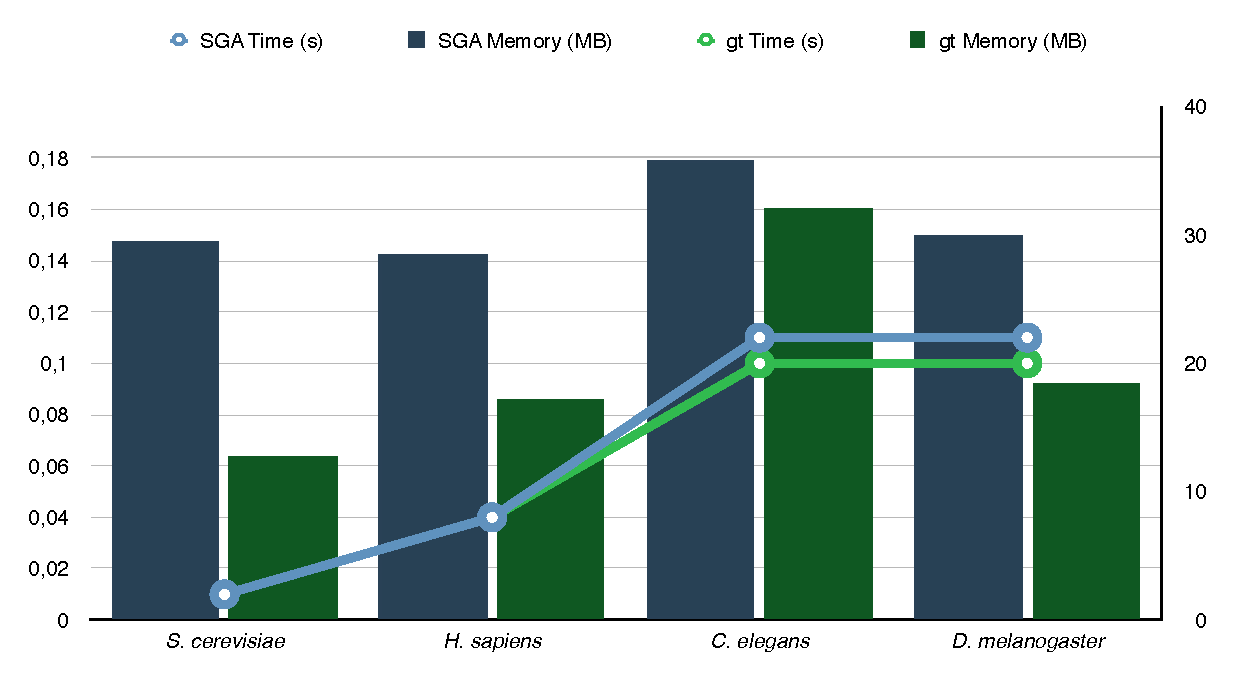
\includegraphics[width=\textwidth,height=0.8\textheight,keepaspectratio]{presentation/figures/sga_vs_gt.pdf}
  \caption{\label{abb: Zeit}Graphische Darstellung der Laufzeit (Graphen) und
  des Speicherplatzbedarfs (Balkendiagramme) von gt Scaffolder (grün) und SGA
  Scaffold (rot) für die nach Größe geordneten Testdatensätze.}
\end{figure}


\subsubsection*{Ergebnisse der Sequenz-Rekonstruktion}
\label{sec: Seq-Rek}
Während gt Scaffolder die Scaffold-Berechnung und Rekonstruktion der
Zielsequenz in einem Schritt berechnen kann, handelt es sich bei SGA
um 2 getrennte Schritte: SGA Scaffold und SGA scaffold2fasta. Für alle
4 Testdatensätze konnte gt Scaffolder eine Sequenz-Rekonstruktion
durchführen. Im Gegensatz zur Scaffold-Berechnung existieren hier
wesentlich Unterschiede zu den mit SGA rekonstruierten Sequenzen
(vgl. Tabelle~\ref{tab: Rekonstruktion}). Die von SGA rekonstruierten
Sequenzen decken das jeweilige Referenzgenom deutlich besser ab und
besitzen gleichzeitig weniger missassemblierte Positionen.

\begin{table}
  \adjustbox{max height=\dimexpr\textheight-5.5cm\relax, max width=\textwidth}{
    \begin{tabular}{llccccc}
      \toprule
      Datensatz & Programm & Länge (Mbp) & Abdeckung (\%) & N50 (kb)
      & \#Miss & Unaligniert (bp) \\
      \midrule
      \textit{S. cerevisiae}
      & SGA scaffold2fasta  & 10.91  &    88.9     &  7.9        &
      2 & 0\\
      & gt Scaffolder & $1.1\times$  & $0.4\times$ & $1.2\times$ &
      $1587.5\times$ & 0\\
      \midrule
      \textit{H. sapiens}, Chr. 21
      & SGA scaffold2fasta  & 34.32  &      73.1   &  54.3       &
      1 & 535\\
      & gt Scaffolder & $0.3\times$  & $0.3\times$ & $0.2\times$ &
      $2114\times$ & $1\times$\\
      \midrule
      \textit{C. elegans}
      & SGA scaffold2fasta  & 94.78  &      90.3   &  37.4       &
      13 & 3301 \\
      & gt Scaffolder & $0.5\times$  & $0.5\times$ & $0.4\times$ &
      $167.9\times$ & $18.2\times$\\
      \midrule
      \textit{D. melanogaster}
      & SGA scaffold2fasta  & 113.50 &      94.2   &  126.4      &
      1  & 0 \\
      & gt Scaffolder & $0.6\times$  & $0.6\times$ & $0.6\times$ &
      $471\times$ & $21871$\\
      \bottomrule
  \end{tabular}}
  \caption{\label{tab: Rekonstruktion}\textbf{Ergebnisse der
      Sequenz-Rekonstruktion.} Die Ergebnisse von SGA sind als absolute Werte aufgetragen,
    die Ergebnisse von gt Scaffolder als relative Faktoren zu ersteren. Wenn ein Wert von
    SGA 0 ist, ist der zugehörige Wert von gt Scaffolder absolut angegeben.
  ~\textit{Länge:} Gesamtlänge aller Scaffolds.
  ~\textit{Abdeckung:} Prozentuale Abdeckung des Refernzgenoms.
  ~\textit{N50:} Länge, sodass alle Scaffolds deren Länge $\geq N50$ mindestens
  die Hälfte der Abdeckung ausmachen.
  ~\textit{\#Miss:} Anzahl der Missassemblierungen nach
  Plantagora~\cite{Gurevich:2013je}.
  ~\textit{Unaligniert:} Anzahl nicht alignierter Basen.}
\end{table}

\subsection{Auswirkung des Auswahlkriteriums für Kantenpaare}
\label{sec: wunderlich_assert}
Wie in Abschnitt~\ref{sec: wunderlich} motiviert, wird im Falle
mehrerer potentieller Kantenpaare bei der Graphkonstruktion das Paar
mit der größten Standardabweichung gewählt. Um die Auswirkung dieses
Kriteriums evaluieren zu können, wurden 2 unterschiedliche Strategien
in gt Scaffolder implementiert: Die beschriebene
MaxStdDev-Strategie und eine MinStdDev-Strategie, bei der das
Kantenpaar mit der geringsten Standardabweichung gewählt
wird. Anschließend wurde die Scaffold-Berechnung mit beiden Strategien
für 4 Testdatensätze (vgl. Tabelle~\ref{sec: Testdaten})
ausgeführt. Dabei wurden nur sehr kleine Unterschiede festgestellt
(vgl.  Tabelle~\ref{tab: stddev}): Die Ergebnisse waren größtenteils
identisch oder wichen zwischen $0.97\times$ und $1.001\times$
voneinandner ab. Zum Zeitpunkt dieser Ausarbeitung ist die
MaxStdDev-Strategie in gt Scaffolder implementiert.

\begin{table}
  \begin{tabular}{llccccc}
    \toprule
    Datensatz & Strategie & Abdeckung (Mbp / \%) & \#Scaf & N50 (kb)\\
    \midrule
    \textit{S. cerevisiae}
    & MaxStdDev  & ~~11.08 / 92  &      ~600   &  32.3      \\
    & MinStdDev  & $0.97\times$     &  $1\times$  & $1\times$    \\
    \midrule
    \textit{H. sapiens}, Chr. 21
    & MaxStdDev  & ~~34.25 / 71  &      1368   &  54.2      \\
    & MinStdDev  & $1\times$     &  $0.99\times$  & $1\times$    \\
    \midrule
    \textit{C. elegans}
    & MaxStdDev  & ~~94.07 / 94  &      5659   &  36.9      \\
    & MinStdDev  & $1\times$     &  $1\times$  & $1\times$    \\
    \midrule
    \textit{D. melanogaster}
    & MaxStdDev  & 113.48 / 81   &      2281   &  126.3     \\
    & MinStdDev  & $1\times$     &  $1.00\times$  & $1.001\times$    \\
    \bottomrule
  \end{tabular}
  \caption{\label{tab: stddev}\textbf{Ergebnisse der Scaffold-Berechnung mit
  verschiedenen Strategien bei der Graphkonstruktion.}
  Die Ergebnisse der MaxStdDev-Strategie sind als absolute Werte aufgetragen, die
  Ergebnisse der MinStdDev-Strategie als relative Faktoren.
  \textit{Abdeckung}, \textit{\#Scaf} und \textit{N50} sind in
  Tabelle~\ref{tab: Scaffolding} erläutert.}
\end{table}

\section{Diskussion}
\label{sec: Diskussion}

\subsection{Scaffold-Berechnung durch gt Scaffolder und SGA im Vergleich}

Wie in Tabelle~\ref{tab: Scaffolding} dargestellt, konnten für die
Scaffold-Berechnung mit gt Scaffolder im Vergleich zu SGA Scaffold
nahezu identische Metriken erzielt werden. Gleichzeitig war der
Laufzeit- und Speicherplatzbedarf leicht bis deutlich geringer.
Hierbei lassen die Ergebnisse der Scaffold-Berechnung keine
Rückschlüsse auf eine Korrelation zwischen der Größe der Zielsequenz
und der Qualität der Ergebnisse zu. Auch die Größe des
Scaffold-Graphen, welche von der Anzahl der eingehenden Contigs
abhängt, scheint keinen Einfluss zu haben. So konnte die größten
Abdeckungen über 90\% für das kleinste (\textit{S.  cerevisiae}, 1694
Contigs) und zweitgrößte (\textit{C. elegans}, 11113 Contigs) der
Referenzgenome erzielt werden.  Die Laufzeit korreliert für die 4
betrachteten Datensätze zwar nicht mit der Größe des Scaffold-Graphen,
steigt jedoch mit der Länge des Zielgenoms an. Der Speicherplatzbedarf
scheint von einer Kombination beider Faktoren abzuhängen und
unterliegt für gt Scaffolder stärkeren Schwankungen als SGA (vgl.
Abbildung~\ref{abb: Zeit}).

Das in gt Scaffolder implementierte Modul zur Sequenz-Rekonstruktion konnte
hingegen keine vergleichbar guten Ergebnisse wie SGA scaffold2fasta liefern
(vgl. Abbildung~\ref{tab: Rekonstruktion}). Dafür kann es verschiedene, mögliche
Ursachen geben: SGA modifiziert den String-Graphen nach dem Einlesen noch
weiter und schließt Lücken zwischen Contigs mit negativer Distanz anhand des
Graphen. Zusätzlich unterscheiden sich die Strategien zur
Alignment-Berechnung. Während gt Scaffolder ein Distanz-Modell verwendet,
nutzt SGA ein Ähnlichkeits-Scoring-Modell, welches übereinstimmende Basen
stärker positiv bewertet. Darüber hinaus kann SGA Contigs ausgeben, welche
nicht im Scaffold enthalten sind. Diese Option (--write-unplaced), welche
gegebenenfalls eine höhere Abdeckung der Zielsequenz erzielen kann, ist in gt
Scaffolder noch nicht implementiert und wurde auch nicht zur
Sequenz-Rekonstruktion verwendet.

\subsection{Evaluation der technischen Implementation}

Sowohl gt Scaffolder (vgl. Abbildung~\ref{abb: help}) als auch SGA
bieten viele vom Nutzer definierbare Parameter und Optionen an. Eine
Vielzahl dieser Parameter ist optional und ermöglicht eine
Feinabstimmung der Scaffold-Berechnung, falls die Standardwerte
unzureichend sind. Lediglich bei der Selektion relevanter Knoten und
Kanten ist SGA flexibler als gt Scaffolder.

gt Scaffolder wurde vollständig in C implementiert. Dies ermöglicht eine hohe
Ausführungsgeschwindigkeit bei geringem Speicherplatzbedarf und einer
vergleichsweise geringen Codegröße von etwas mehr als 200 KB. Das in C++
implementierte SGA Scaffold ist etwa 500 KB groß.

Durch die in den GenomeTools-Bibliotheken vorhandene Datenstrukturen und
Konzepte, wie beispielsweise Arrays, Queues und Hashes, war die Implementierung
ähnlich komfortabel zu einer höheren, objektorientierten Sprache wie C++. Es
konnte ebenfalls auf vorhandene, spezialisierte Algorithmen und
Datenstrukturen zurückgegriffen werden, die unter anderem die Berechung
lokaler Alignments (Smith-Waterman-Algorithmus) oder die Nutzung eines
String-Graphen ermöglichen. Dies stellt neben der höheren
Ausführungsgeschwindigkeit einen wesentlichen Vorteil gegenüber der Nutzung
von Skriptsprachen (Python, Ruby, Perl, $\ldots$) dar. Dort hätten die
vorhandenen Möglichkeiten zur Stringmanipulation hingegen das Einlesen der
Eingabeformate vereinfacht.

\section{Ausblick}
\label{sec: Ausblick}

Die Scaffolding-Software gt Scaffolder kann um weitere Optionen erweitert
werden. Dazu gehört die Implementation weiterer Strategien zur Selektion
relevanter Knoten und Kanten, um eine feinere Abstimmung der Scaffold-
Berechnung zu ermögichen. Beispiele für solche Strategien finden sich in SGA
Scaffold und umfassen eine erweiterte Zyklendetektion oder Entfernung
transitiver Kanten.

Zusätzlich sollten die konservativen Strategien zur Klassifikation
repetitiver bzw.\ eindeutiger Knoten untersucht werden. So sollten die Güte
der entsprechenden Standard-Schwellenwerte evaluiert werden, um potentiell
bessere Ergebnisse erzielen zu können. Einige Strategien von SGA übernommene
Strategien mit unklarer Bedeutung (vgl. Abschnitt~\ref{sec: wunderlich})
müssen darüber hinaus noch überprüft werden.

Obwohl gt Scaffolder einen geringeren Laufzeit- und der Speicherplatzbedarf
als SGA aufweist, lag der Fokus der hier beschriebenen Implementation nicht
auf der Zeit- und Speichereffizienz. Hier stellt die Parallelisierung einiger
Schritte eine Möglichkeit der Laufzeitoptimierung dar. So können die
Scaffolds unabhängig voneinander berechnet werden, da deren Ermittlung für
jede Zusammenhangskomponente separat erfolgt. Die Zyklendetektion und das
darauf folgende eigentliche Scaffolding könnte folglich für jede
Zusammenhangskomponente in einem eigenen Thread stattfinden. Schließlich
könnte die Verwendung effizienterer Datenstrukturen eine Einsparung bei der
Lufzeit und Speicherplatz bewirken.

Die Rekonstruktion der Zielsequenz ist noch verbesserungswürdig (vgl.
Abschnitt~\ref{sec: Rekonstruktion}). Hier können die durch gt Scaffolder
erzeugten Scaffolds im SCAF-Format zur Rekonstruktion genutzt werden. Dazu
könnte eine in SGA bereits implementierte Strategie adaptiert werden.

Zur gemeinsamen Nutzung in einer Pipeline, müssen weitere Anpassungen sowohl
in gt Scaffolder als auch in Readjoiner erfolgen. So müssen die
Informationen über das Mapping der Reads gegenüber den Contigs in das
Standardformat BAM übertragen werden. Dabei könnte Readjoiner um
eine Ausgabe im BAM-Format erweitert oder entsprechendes Umwandlungsskript
für das bestehende Format geschrieben werden. Des Weiteren sollten die
Standardwerte der Parameter nach Fertigstellung der Schnittstelle evaluiert
werden, da die momentan verwendeten Werte aus der SGA-Pipeline stammen.

\section*{Anhang}
\subsection*{Pseudocode}

\begin{algorithm}
  \ForEach{Knoten $k_0$ im Graph $G$}{
    \ForEach{Kantenrichtung $dir$ in [ANTISENSE, SENSE]}{
      \ForEach{Kantenpaar $(e_0,e_1)$ in Richtung $dir$}{
        $k_1$ = $e_0.end$\;
        $k_2$ = $e_1.end$\;
        \If{AmbiguousOrdering($e_0,e_1,p\_cutoff$) \textbf{and}
           $k_1.copy\_num + k_2.copy\_num < cn\_cutoff$}
          {
            \If{$k_1.copy\_num < k_2.copy\_num$}{
              markiere $k_1$ und alle ein- und ausgehenden Kanten
              von $k_1$ als polymorph, wenn $k_1$ noch nicht markiert
              ist\;
            }
            \Else {
              markiere $k_2$ und alle ein- und ausgehenden Kanten
              von $k_2$ als polymorph, wenn $k_2$ noch nicht markiert
              ist\;
            }
          }
        }
      \tcp{polymorphe Knoten müssen nicht mehr auf
        inkonsistente Kanten überprüft werden}
       \If{Knoten $k_0$ ist polymorph}
         {break\;}
       \ForEach{Kantenpaar $(e_0,e_1)$ in Richtung $dir$}{
         \If{$e_0$ ist nicht markiert und $e_1$ ist nicht markiert}
            {
              Berechne Überlappung von $e_0.end$ und $e_1.end$ und speichere
              längsten Überlappung.\;
            }
       }
       \If{längste Überlappung $>$ 400} {
          Markiere alle ausgehenden Sense- bzw. Antisensekanten
          von $k_0$ und die eingehenden Kanten mit der Richtung der
          jeweiligen Zwillingskante als inkonsistent\;
      }
    }
  }
  \caption{\label{alg: Selektion}Filterfunktion zur Markierung von
    polymorphen Knoten und inkonsistenten Kanten. Die Funktion
    \textit{AmbigousOrdering} ist in Algorithmus \ref{alg: Order}
    dargestellt.}
\end{algorithm}

\begin{algorithm}
  \KwData{Kante $e_0$ und Kante $e_1$, die auf eindeutige Ordnung geprüft werden
    sollen. Wahrscheinlichkeitsschwellenwert $p\_cutoff$}
  \KwResult{Ob die Kanten $e_0$ und $e_1$ nicht eindeutig geordnet werden können}
  $\mu = e_0.dist - e_1.dist$\;
  $\sigma^2 = e_0.std\_dev^2 + e_1.std\_dev^2$\;
  $t = \frac{-\mu}{\sigma\cdot\sqrt{2}}$\;
  $P_{e_0,e_1} = \frac{1}{2} \cdot \left( 1 + \frac{2}{\sqrt{\pi}} \int_{0}^{t} \exp{-x^2}\mathrm dx\right)$\;
  $P_{e_1,e_0} = 1 - P_{e_0,e_1}$\;
  \Return $\max\{P_{e_0,e_1}, P_{e_1,e_0}\} \leq p\_cutoff$
  \caption{\label{alg: Order}Funktion \textsc{AmbiguousOrdering}$(e_0, e_1, p\_cutoff)$}
\end{algorithm}

\begin{algorithm}
  \KwData{Graph}
  \KwResult{Graph ohne Zyklen}
  \While{Zyklus gefunden wurde}{
  Suche alle Zusammenhangskomponenten $CC$\;
  \ForEach{Zusammenhangskomponente $C_0 \in CC$}{
    Suche alle terminalen Knoten $T$\;
    \ForEach{terminalen Knoten $t_0 \in T$}{
      Suche mit einer Tiefensuche von dem Knoten $t_0$ aus in der
      Richtung $t_0.edges[0].sense$ nach Rückkanten\;
      \If{Rückkante gefunden}{
        Markiere die Rückkante und die dadurch verbundenen Knoten
        als zyklisch\;
        }
      }
    }
  }
  \caption{\label{alg: Zyklen}Löse alle Zyklen für jede
    Zusammenhangskomponente auf}
\end{algorithm}

\begin{algorithm}
  \SetAlgoLined
  \KwData{Graph $G$}
  \KwResult{Graph $G$ mit Knoten der Scaffolds markiert}
  Suche alle Zusammenhangskomponenten $CC$\;
  \ForEach{Zusammenhangskomponente $C_0\in CC$}{
    Berechne die Menge der terminalen Knoten $T$ für $C_0$\;
    \ForEach{terminalen Knoten $t_0  \in T$}{
      Berechne die Menge $W$ aller Pfade durch $C_0$ von $t_0$ aus\;
      \ForEach{Pfad $w_0$ aus $W$}{
        \If{Contig-Gesamtlänge > bislang beste Contig-Gesamtlänge}{
          Setze aktuellen Pfad $w_0$ als besten Pfad\;
        }
      }
    }
    Markiere alle Knoten und Kanten entlang des besten Pfades als Scaffold\;
  }
  \caption{\label{alg: Scaffold}Berechnung der Scaffolds. Die
    Berechnung aller Pfade ist in Algorithmus \ref{alg: Pfade} dargestellt.}
\end{algorithm}

\begin{algorithm}
  \SetAlgoLined
  \KwData{terminaler Startknoten $t_0$}
  \KwResult{Alle von diesem Knoten möglichen Pfade}
  Konstruktionsrichtung = $t_0.edges[0].sense$\;
  \ForEach{Kante $e_1$ vom Knoten $t_0$ ausgehend}{
    $k_0$ = $e_1.end$\;
    Speichere Startkante $e_1$ und Distanz $e_1.dist$ in Map an Position
    $k_0$\;
    Schiebe Startkante $e_1$ und Distanz $e_1.dist$ in Queue\;
  }
  \While{BFS über Queue nicht beendet}{
    Poppe Kante $e$ und Distanz $dist$ aus der Queue\;
    $k$ = $e.end$\;
    \ForEach{Kante $e_2$ in Konstruktionsrichtung von $k$ aus} {
      $k_1$ = $e_2.end$\;
      \If{Distanz ($e_2.dist + dist$) zu aktuell betrachtetem Knoten $k_1$ $<$
        bisher ermittelte Distanz zu $k_1$ {\bf OR} Knoten $k_1$
        noch unbetrachtet}{
        Speichere Kante $e_2$ und Distanz $e_2.dist + dist$ in Map an Position $k_1$\;
        Schiebe Kante $e_2$ und Distanz $e_2.dist + dist$ in Queue\;
      }
      neue Konstruktionrichtung = $e_2.twin.sense$\;
    }
    \If{$k$ hat keine Kanten in Konstruktionsrichtung {\bf AND}
    $k$ ist terminal}{
      Schiebe Knoten $k$ in terminalSet $S$\;
    }
  }
  \ForEach{Knoten $k\in S$}{
    Erzeuge Pfad von $t_0$ zu $k$ mithilfe einer Rücktraversierung über die Map\;
  }
  \caption{\label{alg: Pfade}Berechnung aller Pfad zwischen einem
    terminalen Knoten und allen anderen terminalen Knoten einer
    Zusammenhangskomponente}
\end{algorithm}

\bibliography{presentation/literatur}
\bibliographystyle{alphadin}

\end{document}
